% this file is called up by thesis.tex
% content in this file will be fed into the main document

%: ----------------------- name of chapter  -------------------------
\chapter{A Hybrid Gaussian-HMM-Deep-Learning Approach}\label{cp:ghmm} % top level followed by section, subsection


As recapped in Section~\ref{sec:3-2-rnnpm}, by now there are basically three types of deep learning approach for ACE:
\begin{itemize}
\item local classification - global smoothing \cite{humphrey2012rethinking};
\item local feature learning - global classification - global smoothing \cite{boulanger2013audio,sigtia2015audio};
\item local feature learning - local classification - global smoothing \cite{zhou2015chord}.
\end{itemize}
All these approaches apply similar deep learning methodologies in ASR \cite{deng2014deep,bourlard2012connectionist} directly to ACE, but they overlook a fundamental difference, that chords are usually segmented rhythmically and they are sustaining much longer than phonemes. This crucial divergence could allow some different approaches for ACE.

This chapter introduces a new approach that leverages this property of ACE. Particularly, the method described here can be categorized as ``local feature extraction - global segmentation - local classification'', which isolates the process of segmentation from classification, and only performs the latter within each segmented region. 

Note that in recent MIREX ACE submissions, systems' segmentation qualities are fairly comparable with each other \cite{burgoyne2014comparative}, and all these systems perform segmentation and classification in one single pass at the same time, which leads to the belief that setting apart the two will bring more benefit to system performance.

%: ----------------------- contents from here ------------------------

\section{System Framework} \label{sec:3-sysframe}

Figure~\ref{fig:3-sysover} depicts the ACE system framework considered in our study. The workflow is as follows%The training process is as follows:
\begin{enumerate}
	
	\item Both training and testing data share the same feature extraction module. Features are extracted from each input track using a method similar to the one employed in the Chordino system~\cite{mauch2010automatic} (will be elaborated in Section~\ref{sec:3-chordino-like fe}).
	\item For training, the feature sequence is segmented (in terms of chords) by ground truth annotations. For testing, the feature sequence is segmented using a GMM-HMM process (will be discussed in Section~\ref{sec:3-chordino-like sg}).
	\item Each feature segment is tiled into a fixed number of sub-segments (see Section~\ref{sec:3-seg-tile}).
	\item For training, the sub-segments together with the segment's chord label, are considered as one sample to train the deep neural nets (will be described in Section~\ref{sec:3-dlmodel}). For testing, the already trained model is used to predict chord labels.
	
\end{enumerate}


\begin{figure}
\centering
\includegraphics[width=0.5\columnwidth]{3/figures/sys.pdf}
\caption{GMM-HMM ACE System framework.}
\label{fig:3-sysover}
\end{figure}

\subsection{Feature Extraction} \label{sec:3-chordino-like fe}
Feature extraction starts with resampling the raw audio input at 11025 Hz, followed by transforming it using short-time-Fourier-transform (STFT) with 4096-point Hamming window and 512-point hop size. The process then proceeds to transform the linear-frequency-scale spectrogram (2049-bin) to log-frequency-scale (252-bin, 3 bins per semitone ranging from MIDI note 21 to 104). And then it tunes the spectrogram to standard tuning using equation~\ref{eq:3-2-tuning}. To enhance harmonic content and attenuate background noise, a standardization process is performed by running-mean subtraction and running-standard-deviation division along the frequency bins: %** according to R1, this is not elaborated in detail, now it is.
\begin{equation}
	Y^{STD}_{k,m} = 
	\begin{cases}
		{{Y_{k,m} - \mu_{k,m}} \over \sigma_{k,m}}, \text{\quad\quad\quad if } Y_{k,m} > \mu_{k,m}\\
		0 \quad\quad\quad\quad\quad\quad\quad\quad\quad\text{otherwise,}
	\end{cases}
\end{equation}
where $\mu_{k,m}$ and $\sigma_{k,m}$ are the mean and standard deviation of the half-octave window of bins centered at $Y_{k,m}$, respectively. This is followed by an NNLS method  (equation~\ref{eq:3-2-nnls}) to extract note activation patterns (84-bin, 1 bin per semitone) \cite{mauch2010approximate}. This matrix is further reduced to a 24-bin per column bass-treble chromagram weighted by the bass and treble profiles (Figure~\ref{fig:3-btprofile}). Each chroma is normalized by its maximum norm. Table~\ref{tab:3-felevels} provides a summary of different levels of features generated by this process. Note that for brevity, in the following tuned notegram is referred to as as ``-ns'', NNLS notegram as ``-nnls'' and chromagram (or bass-treble chromagram) as ``-ch''.

\begin{figure}[htb]
\centering
\includegraphics[width=0.5\columnwidth]{3/figures/btp.pdf}
\caption{Bass (+) and treble (.) profiles. They are both computed in the shape of Rayleigh distributions with scale parameters 16.8 (for bass) and 42 (for treble) respectively. The horizontal axis stands for MIDI pitch numbers. The vertical axis represents normalized profile amplitudes from 0 to 1.}
\label{fig:3-btprofile}
\end{figure}
% The bass profile is computed as a Rayleigh distribution in order to allow more high range salience to get in.

\begin{table}[htb]
\caption{Different levels of feature representations}
\centering
\footnotesize
\begin{tabular}{|c|c|c|} \hline
 Process & Output level & Bins \\ \hline
 STFT & spectrogram & 2049 \\ \hline
 Linear-Log Mapping & notegram & 252  \\ \hline
 Tuning & tuned notegram (-ns) & 252 \\ \hline
 NNLS & NNLS notegram (-nnls) & 84  \\ \hline
 Bass-treble Profiling & chromagram (-ch) & 24 \\ \hline
\end{tabular}
\label{tab:3-felevels}
\end{table}

Here are some simple showcases of the feature extraction process output at notegram level. All of them are extracted from acoustic piano audio.

Figure~\ref{fig:3-note_C} illustrates the notegram of a middle C note, Figure~\ref{fig:3-interval_CE} a major third interval built upon the middle C, and Figure~\ref{fig:3-chord_Cmaj} a C major chord rooted on the same note. Note the appearance of the harmonics and background noise.

\begin{figure}
\centering
\includegraphics[width=0.6\columnwidth]{3/figures/note_C.pdf}
\caption{Middle C note - notegram}
\label{fig:3-note_C}
\end{figure}

\begin{figure}
\centering
\includegraphics[width=0.6\columnwidth]{3/figures/interval_CE.pdf}
\caption{Major third interval - notegram}
\label{fig:3-interval_CE}
\end{figure}

\begin{figure}
\centering
\includegraphics[width=0.6\columnwidth]{3/figures/chord_Cmaj.pdf}
\caption{C major chord - notegram}
\label{fig:3-chord_Cmaj}
\end{figure}

The above are all simple music elements with pure pitches. Figure~\ref{fig:3-cp} is a notegram example of the intro (first few seconds) of {\it Let it be} . As this is just a piano intro, no vocal melody is involved. Note how it is rhythmically segmented.
\begin{figure}
\centering
\includegraphics[width=0.5\columnwidth]{3/figures/cp.png}
\caption{Chord progression example - notegram}
\label{fig:3-cp}
\end{figure}
Figure~\ref{fig:3-cpm} showcases a symmetrical example with vocal melody. It is extracted from the first line of the first verse. Note although this is much more corrupted, a rhythmical segmentation is also visually noticeable.
\begin{figure}
\centering
\includegraphics[width=0.5\columnwidth]{3/figures/cpm.png}
\caption{Chord progression with vocal melody example - notegram}
\label{fig:3-cpm}
\end{figure}

\newpage
\subsection{Segmentation} \label{sec:3-chordino-like sg}
Similar to \cite{cannam2013mirex}, the segmentation process is implemented as an expert knowledge driven GMM-HMM (as shown in Figure~\ref{fig:3-hmm1}), which is characterized as follows:
\begin{itemize}
\item The hidden node models discrete states of categorical chord classes.
\item The observable node represents continuous states of a chroma.
\item The emission probabilities are designed as a 24-dimension Gaussian distribution with parameters shown in Table~\ref{tab:3-gaussian}.
\item The transition matrix is set with a heavy uniform self-transition weight, which is more than 99 times of the uniform non-self-transition weight. 
\item The prior matrix is uniform.
\end{itemize}

\begin{table}
\caption{Segmentation parameters.}
\centering
\footnotesize
\begin{tabular}{|c|c|c|} \hline
      & $\mu$ & $\sigma^2$ \\ \hline
 Bass - chord bass & 1 & 0.1 \\ \hline
 Bass - not chord bass but chord note & 1 & 0.5  \\ \hline
 Bass - not bass & 0 & 0.1 \\ \hline
 Treble - chord note & 1 & 0.2  \\ \hline
 Treble - not chord note & 0 & 0.2 \\ \hline
 No Chord (for all notes)  & 1 & 0.2  \\ \hline
\end{tabular}
\label{tab:3-gaussian}
\end{table}

\begin{figure}[htb]
\centering
\includegraphics[width=0.4\columnwidth]{3/figures/hmm1.pdf}
\caption{GMM-HMM Segmentation.}
\label{fig:3-hmm1}
\end{figure}

Figure~\ref{fig:3-cdflow} summarizes the full information flow of the above feature extraction and segmentation process using the first line of {\it Let it be}. Note how representations are enhanced or compressed during this process.
\begin{figure}[h]
\centering
\includegraphics[width=1\columnwidth,angle =90]{3/figures/cdflow.pdf}
\caption{Information flow of feature extraction and segmentation}
\label{fig:3-cdflow}
\end{figure}

\subsection{Segment Tiling Process} \label{sec:3-seg-tile}

The segment tiling process is introduced to equalize the length of every segment, so as to facilitate the use of neural network models with fixed length input. This process divides a segment into $N$ equal-sized sub-segments, and takes the average feature of each sub-segment, resulting in a $N$-frame segment. If the original number of frames is not divisible by $N$, the last frame is extended to make it divisible. In a word, this process turns a segment with variable number of frames into a segment with $N$ frames.

\subsection{Deep Learning Models} \label{sec:3-dlmodel}

Each $N$-frame segment is classified as a chord label through a deep learning model. Three types of model are considered: DBN, MLP, and RNN.

\subsubsection{Deep Belief Network}

The DBN, as shown in Figure~\ref{fig:3-dbn} models the chord posteriors conditioned on the tiled chromagram. In this model, the RBM formed by the input layer and the first hidden layer is a Gaussian-Bernoulli RBM because the input feature (chromagram) is in continuous value space. The RBMs formed by hidden layer pairs are Bernoulli-Bernoulli RBMs, since each neuron is stochastic binary \cite{hinton2006reducing}. In the fine-tuning phase, the network is regarded as a MLP and trained via SGD with back-propagation.

\begin{figure}[htb]
\centering
\includegraphics[width=0.4\columnwidth]{3/figures/dbn.pdf}
\caption{The deep belief network architecture used in our system. All layers are fully connected. The input is N-frame of features.}
\label{fig:3-dbn}
\end{figure}

\subsubsection{Multilayer Perceptrons}
The MLP model has the same bottom-up topology as the DBN model, but it is without the top-down generative connections. It is trained via SGD with back-propagation.

\subsubsection{Recurrent Neural Network}

The RNN shown in Figure~\ref{fig:3-rnn} is bidirectional with LSTM hidden units \cite{hochreiter1997long}, or it can be called a BLSTM-RNN. As recapped in chapter~\ref{cp:background}, LSTM is introduced in order to relieve gradient vanishing/exploding problem for long sequence training \cite{bengio2009learning}. For a fixed length $N$-frame input, the RNN is expanded to $N$ frames, each taking one frame of input. A mean pooling operation \cite{maas2011learning}, similar to those normally used in a CNN \cite{lecun1995convolutional}, is inserted before the output layer to summarize the LSTM activations of all frames.
\begin{figure}[h]
\centering
\includegraphics[width=0.6\columnwidth]{3/figures/rnn.pdf}
\caption{The bidirectional recurrent neural network architecture used in our system. Both hidden layers employ LSTM units in place of normal logistic units. The RNN is expanded to N frames, with mean pooling to summarize results.}
\label{fig:3-rnn}
\end{figure}

\section{Experiments} \label{sec:3-exper}
This section describes a systematic approach to sample the design space of the ACE framework. All system configurations are tested under the same benchmark. %First the datasets is introduced, and then the design space sampling scheme is elaborated. This section is ended by expounding the training and testing process.

\subsection{Datasets}
For training/validation, five datasets of 366 tracks in total are used. They contain both eastern and western pop/rock songs. They are:
\begin{itemize}
\item JayChou29 (J) dataset \cite{deng2016chord}, annotated by the author of this thesis \footnote{\url{http://www.tangkk.net/label/}};
\item a Chinese pop song dataset (CNPop20, or C) \footnote{containing 20 songs from both male and female singer-songwriters from Chinese cultural backgrounds}, also annotated by the author \cite{deng2016hybrid};
\item Carole King + Queen dataset (KingQueen26, or K) \footnote{\url{http://isophonics.net/datasets}}, annotated by Mauch \cite{mauch2009omras2} in C4DM (Center for Digital Music in Queen Mary University of London);
\item 191 songs from USPop dataset (U) \footnote{\url{http://labrosa.ee.columbia.edu/projects/musicsim/uspop2002.html}}, annotated by MARL (Music and Audio Research Lab in New York University) \footnote{\url{https://github.com/tmc323/Chord-Annotations}} \cite{cho2014improved};
\item 100 songs from RWC dataset, provided by the RWC group \footnote{\url{https://staff.aist.go.jp/m.goto/RWC-MDB/}} and also annotated by MARL \cite{cho2014improved}.
\end{itemize}
The combination of datasets is notated by concatenating their letter codes. For example, a combination of all training datasets is denoted as ``CJKU''. These notations will be used extensively in Section~\ref{sec:3-res}.

Each track is extracted at both bass-treble chromagram (-ch) and tuned notegram (-ns) level. The features at these two levels can be transposed to all 12 different keys by circular pitch shifting (for -ch) or pitch shifting with zero padding (for -ns). For example, for a piece of treble chromagram in key of $C$, the original treble pitch class profile (PCP) $PCP_C$ = ($C'$,$C\#'$, $D'$, $D\#'$, $E'$, $F'$, $F\#'$, $G'$, $G\#'$, $A'$, $A\#'$, $B'$), where $X'$ stands for the salience of the pitch class $X$, can be circular shifted to represent an equivalent PCP in other keys, such as key of $D$: $PCP_D$ = ($D'$, $D\#'$, $E'$, $F'$, $F\#'$, $G'$, $G\#'$, $A'$, $A\#'$, $B'$, $C'$,$C\#'$). The same process can also be conducted for bass chromagrams. As for tuned notegram, since the saliences are presented in terms of pitches rather than in pitch classes, the saliences in high-pitch range cannot be ``circulated'' to low-pitch range, vice versa, but the same ``pitch shifting'' ideas can be applied to make equivalent features in other keys, only that the out-shifted positions are filled by zeros rather than the circulated saliences. In practice, the original key is considered as a pivot, and the features are transposed to all other 11 keys by -6 to 5 semitones circular shifting. Adjusting the ground truth labels accordingly, this results in a 12-time data augmentation, which helps in reducing over-fitting \cite{cho2014improved,humphrey2015exploration}. This is commonly considered as a type of regularization.

TheBeatles180 (B) dataset is used for testing. It is annotated by Harte \cite{harte2010towards}, who refers to Pollack's previous chord transcriptions \cite{pollack2000notes}. It measures how well a system generalizes outside the scope of data that it has been trained on. Here cross-validation is not used because of the following reasons. Firstly, one of the major missions of this work is to explore the design space of the proposed system framework. If cross-validation is employed, it is difficult to observe the effect of increasing training data size. More importantly, the models are trained NOT with whole labeled tracks, but labeled ``segments'', but the validation should be run on whole tracks, not segments. This leaves the cross-validation scheme problematic to be used. Lastly, it is unsure whether cross-validation results can be directly compared with the performance of an expert system.

\subsection{Design Space Sampling}
There is a large design space under the system framework. Specifically, possible dimensions include:
\begin{itemize}
\item choice of deep learning model; 
\item depth and width of hidden layers (network configurations);
\item number of frames in segment tiling;
\item input feature representation level; and
\item training data size.
\end{itemize}

\begin{table}
\caption{Variations considered in this study.}
\centering
\footnotesize
\begin{tabular}{|c|c|c|} \hline
Dimension & Configurations to Try \\ \hline
model & MLP; DBN; BLSTM-RNN \\ \hline
N-frame & 1; 2; 3; 6; 9; 12 \\ \hline
layer depth & 2; 3; 4; 5 \\ \hline
layer width & 500; 800; 1000; 2000 \\ \hline
input representation & tuned notegram (-ns); chromagram (-ch) \\ \hline
training data size & J; CJK; CJKU \\ \hline
\end{tabular}
\label{tab:3-varexplore}
\end{table}

This study is based on the settings depicted in Table~\ref{tab:3-varexplore}. Indeed, it is impractical to sample all combinations. A more practical yet systematic method is proposed, which samples one dimension at a time with all other dimensions fixed at a previously explored point. If a dimension is not yet explored, a random choice of value is used.

Specifically, the scheme first samples along the {\it layer width}, and then along the {\it layer depth}. After understanding the two variations, the segment tiling scheme will be explored with fixed {\it layer width} and {\it layer depth}. Following this same strategy, all factors in Table~\ref{tab:3-varexplore} are explored. It is important to note that neither does this process lead to a full picture of the design space, nor does it lead to optimality, but it gains us some significant insights.

%The concrete samples and their performances will be discussed in Section \ref{sec:3-res}.

\subsection{Training and Testing} \label{sec:3-traintest}

To control variations of training, the following techniques are applied in all implementations. 
\begin{itemize}
\item An MLP model is trained using mini-batch stochastic gradient descent regularized with dropout \cite{srivastava2014dropout} and early-stopping \cite{prechelt1998automatic}. 
\item A DBN model is pre-trained using persistent-contrastive-divergence \cite{tieleman2008training} (PCD-20), for 100 epochs with learning rate 0.001. It is fine-tuned using mini-batch stochastic gradient descent regularized with dropout and early-stopping.
\item During mini-batch stochastic gradient descent, both MLP and DBN use a learning rate of 0.01 and a batch size of 100. 
\item A BLSTM-RNN model is trained using an Adadelta optimizer \cite{zeiler2012adadelta}, regularized with dropout and early-stopping. 
\item All dropout probabilities are set to 0.5. 
\item The early-stopping event is cross-checked by a validation set, which is a random choice of 20\% of the training dataset, while the other 80\% are used for computing gradients and updating the network.
\end{itemize}

In the testing process, each of the 180 tracks in the test dataset are chord estimated from raw audio file. The output is written in a {\tt .lab} file conforming with the ``start\_time end\_time chord'' format \footnote{\url{http://www.music-ir.org/mirex/wiki/2016:Audio\_Chord\_Estimation}}, where the ``chord'' is conforming with Harte's format \cite{harte2005symbolic}. All implementation details are available online \footnote{\url{github.com/tangkk/tangkkace}} in so that interested readers can repeat the experiments. All deep learning components are implemented under Theano framework \cite{bergstra2010theano}.

\subsection{Network configurations} \label{sec:3-p2}

\pgfplotsset{width=8cm,height=4cm,every node near coord/.append style={font=\scriptsize}}
\begin{figure}[htb]
	\centering
	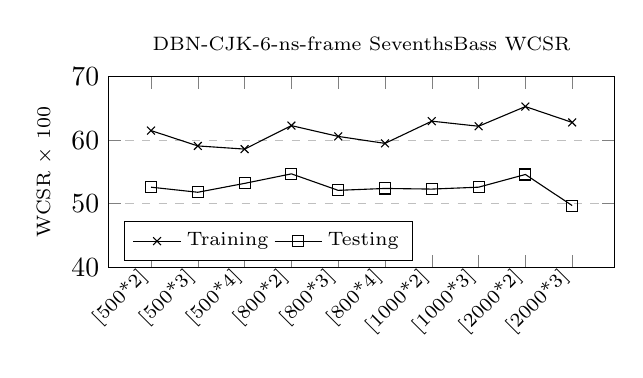
\begin{tikzpicture}
	\begin{axis}[
	title={DBN-CJK-6-ns-frame SeventhsBass WCSR},
	title style = {font=\scriptsize},
	%xlabel={Network Configuration},
	x label style={font=\scriptsize},
	symbolic x coords={[500*2],[500*3],[500*4],[800*2],[800*3],[800*4],[1000*2],[1000*3],[2000*2],[2000*3]},
	x tick label style={rotate=45,anchor=east, font=\scriptsize},
	xtick=data,
	ylabel={WCSR $\times$ 100},
	y label style={font=\scriptsize},
	ymin=40, ymax=70,
	ytick={40,50,60,70},
	legend pos=south west,
	legend style={legend columns=-1, font=\scriptsize},
	ymajorgrids=true,
	grid style=dashed,
	]
	\addplot[
	color=black,
	mark=x,
	]
	coordinates {
		([500*2],61.52)([500*3],59.1)([500*4],58.6)([800*2],62.3)([800*3],60.6)([800*4],59.5)([1000*2],63.0)([1000*3],62.2)([2000*2],65.3)([2000*3],62.8)
	};
	
	\addplot[
	color=black,
	mark=square,
	]
	coordinates {
		([500*2],52.6)([500*3],51.8)([500*4],53.2)([800*2],54.7)([800*3],52.1)([800*4],52.4)([1000*2],52.3)([1000*3],52.6)([2000*2],54.6)([2000*3],49.7)
	};
	\legend{Training, Testing} 
	\end{axis}
	\end{tikzpicture}
	\caption{Exploring different DBN-ns network configurations. All systems are trained with CJK-6-ns-frame.}
	\label{fig:3-dbn-ns-configs}
\end{figure}

% ** R3: would be interesting to see training set numbers too (also for some other plots)
\Hsection{-ns level}
Figure~\ref{fig:3-dbn-ns-configs} shows the scores of ten DBN-ns systems with different network configurations. They have 2, 3 or 4 hidden layers with 500, 800, 1000 or 2000 neurons per layer. Within all these configurations [800*2] achieves the best testing score, followed by [2000*2]. As the layer width becomes larger the model fits better to the training data, but as the layer depth goes larger, the model unexpectedly fits worse. It seems the strong pre-training regularization does not compensate enough for the gradient vanishing of a deeper model. The results indicate that, firstly, in terms of DBN-ns systems, a two-hidden-layer network performs better than or at least as good as a deeper architecture with the same layer width. Secondly, under the current settings, DBN model capacity could be increased by layer width instead of layer depth.

\pgfplotsset{width=8cm,height=4cm,every node near coord/.append style={font=\scriptsize}}
\begin{figure}[htb]
	\centering
	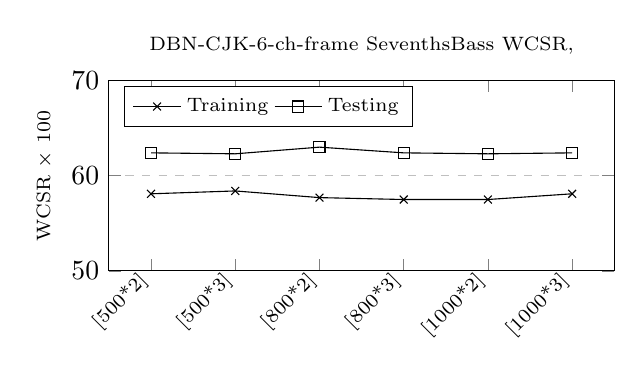
\begin{tikzpicture}
	\begin{axis}[
	title={DBN-CJK-6-ch-frame SeventhsBass WCSR,},
	title style = {font=\scriptsize},
	%xlabel={Network Configuration},
	x label style={font=\scriptsize},
	symbolic x coords={[500*2],[500*3],[800*2],[800*3],[1000*2],[1000*3]},
	x tick label style={rotate=45,anchor=east, font=\scriptsize},
	xtick=data,
	ylabel={WCSR $\times$ 100},
	y label style={font=\scriptsize},
	ymin=50, ymax=70,
	ytick={50,60,70},
	legend pos=north west,
	legend style={legend columns=-1, font=\scriptsize},
	ymajorgrids=true,
	grid style=dashed,
	]
	
	\addplot[
	color=black,
	mark=x,
	]
	coordinates {
		([500*2],58.1)([500*3],58.4)([800*2],57.7)([800*3],57.5)([1000*2],57.5)([1000*3],58.1)
	};
	
	\addplot[
	color=black,
	mark=square,
	]
	coordinates {
		([500*2],62.4)([500*3],62.30)([800*2],63.0)([800*3],62.4)([1000*2],62.3)([1000*3],62.4)
	};
	\legend{Training, Testing} 
	\end{axis}
	\end{tikzpicture}
	\caption{Exploring different DBN-ch network configurations. All systems are trained with CJK-6-ch-frame.}
	\label{fig:3-dbn-ch-configs}
\end{figure}

\Hsection{-ch level}
Figure~\ref{fig:3-dbn-ch-configs} shows scores of DBN-ch systems with different network configurations. First of all, it is interesting to notice that, different from the DBN-ns results, all the training scores here are lower than the testing scores, and the training scores do not show any trend of decreasing with the growing of network complexity, which indicates a very strong bias. As these variants differ from those in the previous subsection only in the choice of feature, it is highly assured that the main bias comes from the feature itself, which is the bass-treble chromagram. The bias is introduced from the manually designed process of transforming tuned notegram (-ns) to bass-treble chromagram (-ch). On one hand, this bias is highly effective as the testing scores of these ``-ch'' systems are all much higher than the ``-ns'' systems in the previous subsection, but on the other hand, it seems compared with ``-ns'' there is much less room for improvement using ``-ch'' features for deep learning.

Given that in all the previous experiments both DBN-ch and DBN-ns peak at [800*2], this configuration is chosen as a default for the following experiments. Note that optimality is not a central issue in this discussion.

\subsection{Segment tiling} \label{sec:3-p3}

\pgfplotsset{width=8cm,height=4cm,every node near coord/.append style={font=\scriptsize}}
\begin{figure}[htb]
	\centering
	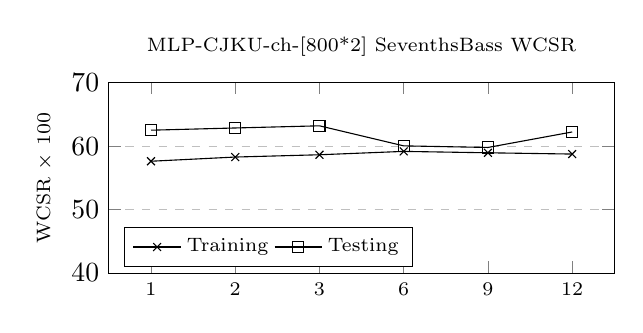
\begin{tikzpicture}
	\begin{axis}[
	title={MLP-CJKU-ch-[800*2] SeventhsBass WCSR},
	title style = {font=\scriptsize},
	x label style={font=\scriptsize},
	symbolic x coords={1,2,3,6,9,12},
	x tick label style={font=\scriptsize},
	xtick=data,
	ylabel={WCSR $\times$ 100},
	y label style={font=\scriptsize},
	ymin=40, ymax=70,
	ytick={40,50,60,70},
	legend pos=south west,
	legend style={legend columns=-1, font=\scriptsize},
	ymajorgrids=true,
	grid style=dashed,
	]
	\addplot[ % Training
	color=black,
	mark=x,
	]
	coordinates {
		(1,57.62)(2,58.28)(3,58.64)(6,59.17)(9,58.95)(12,58.75)
	};
	
	\addplot[ % Testing
	color=black,
	mark=square,
	]
	coordinates {
		(1,62.51)(2,62.86)(3,63.20)(6,60.04)(9,59.79)(12,62.23)
	};
	\legend{Training, Testing} 
	\end{axis}
	\end{tikzpicture}
	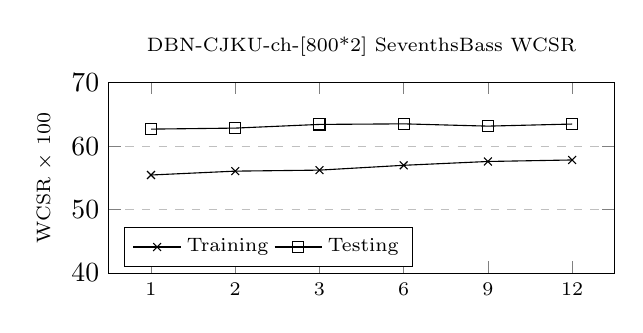
\begin{tikzpicture}
	\begin{axis}[
	title={DBN-CJKU-ch-[800*2] SeventhsBass WCSR},
	title style = {font=\scriptsize},
	x label style={font=\scriptsize},
	symbolic x coords={1,2,3,6,9,12},
	x tick label style={font=\scriptsize},
	xtick=data,
	ylabel={WCSR $\times$ 100},
	y label style={font=\scriptsize},
	ymin=40, ymax=70,
	ytick={40,50,60,70},
	legend pos=south west,
	legend style={legend columns=-1, font=\scriptsize},
	ymajorgrids=true,
	grid style=dashed,
	]
	\addplot[ % Training
	color=black,
	mark=x,
	]
	coordinates {
		(1,55.45)(2,56.06)(3,56.22)(6,56.98)(9,57.58)(12,57.82 )
	};
	
	\addplot[ % Testing
	color=black,
	mark=square,
	]
	coordinates {
		(1,62.68)(2,62.84)(3,63.42)(6,63.51)(9,63.15)(12,63.48)
	};
	\legend{Training, Testing} 
	\end{axis}
	\end{tikzpicture}
	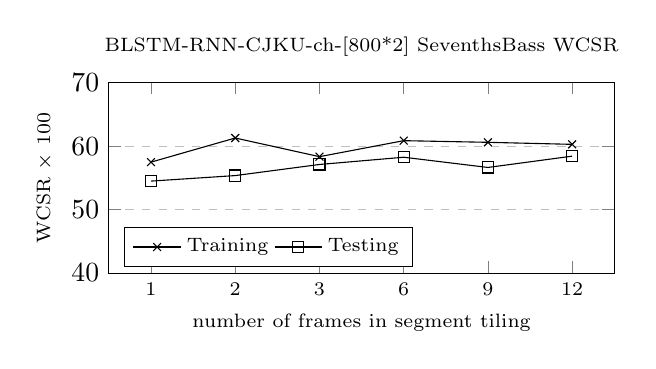
\begin{tikzpicture}
	\begin{axis}[
	title={BLSTM-RNN-CJKU-ch-[800*2] SeventhsBass WCSR},
	title style = {font=\scriptsize},
	x label style={font=\scriptsize},
	symbolic x coords={1,2,3,6,9,12},
	x tick label style={font=\scriptsize},
	xtick=data,
	xlabel={number of frames in segment tiling},
	ylabel={WCSR $\times$ 100},
	y label style={font=\scriptsize},
	ymin=40, ymax=70,
	ytick={40,50,60,70},
	legend pos=south west,
	legend style={legend columns=-1, font=\scriptsize},
	ymajorgrids=true,
	grid style=dashed,
	]
	\addplot[ % Training
	color=black,
	mark=x,
	]
	coordinates {
		(1,57.48)(2,61.28)(3,58.34)(6,60.86)(9,60.60)(12,60.28)
	};
	
	\addplot[ % Testing
	color=black,
	mark=square,
	]
	coordinates {
		(1,54.49)(2,55.36)(3,57.11)(6,58.25)(9,56.64)(12,58.42)
	};
	\legend{Training, Testing} 
	\end{axis}
	\end{tikzpicture}
	\caption{Exploring effect of segment tiling. All systems are trained with CJKU-ch-[800*2]}
	\label{fig:3-N-frame}
\end{figure}

\Hsection{-ch level}
A set of systems are implemented using CJKU-ch-[800*2] with different $N$-frame segment tiling. The [800*2] in BLSTM-RNN means there are one forward and one backward hidden layer, each having 800 LSTM units.

As shown in Figure~\ref{fig:3-N-frame}, similar to DBN-ch's case in the above subsection, both MLP and DBN have higher testing scores than training scores, and their scores hardly change from 1-frame to 12-frame segment tiling. This is still because the -ch feature itself has already introduced a very strong prior knowledge, that the distribution of pitch saliences over different octaves of a pitch class is irrelevant in classifying a chord. The regularized MLP and DBN models do not have large enough flexibilities to learn something that could overcome the bias. Since DBN has much stronger regularization than MLP, it is also much more unchangeable than MLP.

As for BLSTM-RNN, it has a normal behavior that training scores are higher than testing scores, which means the model flexibility to some extent offsets the high bias imposed by the low dimensional features. As ``N'' goes larger, the model complexity increases, and so does the testing score, because the model is approaching a better bias-variance trade-off point. But it turns out the overall testing performances of BLSTM-RNN in Figure~\ref{fig:3-N-frame} are far lower than the other two models. This will be further discussed in Section~\ref{sec:3-p5}.

\pgfplotsset{width=8cm,height=4cm,every node near coord/.append style={font=\scriptsize}}
\begin{figure}[htb]
	\centering
	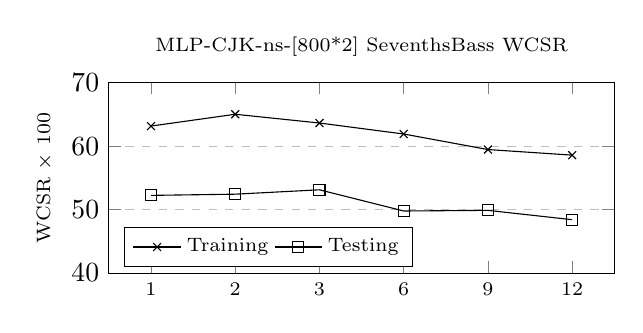
\begin{tikzpicture}
	\begin{axis}[
	title={MLP-CJK-ns-[800*2] SeventhsBass WCSR},
	title style = {font=\scriptsize},
	x label style={font=\scriptsize},
	symbolic x coords={1,2,3,6,9,12},
	x tick label style={font=\scriptsize},
	xtick=data,
	ylabel={WCSR $\times$ 100},
	y label style={font=\scriptsize},
	ymin=40, ymax=70,
	ytick={40,50,60,70},
	legend pos=south west,
	legend style={legend columns=-1, font=\scriptsize},
	ymajorgrids=true,
	grid style=dashed,
	]
	\addplot[ % Training
	color=black,
	mark=x,
	]
	coordinates {
		(1,63.16)(2,65.02)(3,63.64)(6,61.91)(9,59.46)(12,58.58)
	};
	
	\addplot[ % Testing
	color=black,
	mark=square,
	]
	coordinates {
		(1,52.24)(2,52.43)(3,53.12)(6,49.78)(9,49.88)(12,48.41)
	};
	\legend{Training, Testing} 
	\end{axis}
	\end{tikzpicture}
	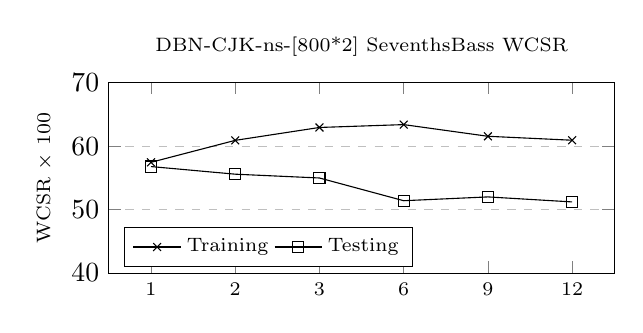
\begin{tikzpicture}
	\begin{axis}[
	title={DBN-CJK-ns-[800*2] SeventhsBass WCSR},
	title style = {font=\scriptsize},
	x label style={font=\scriptsize},
	symbolic x coords={1,2,3,6,9,12},
	x tick label style={font=\scriptsize},
	xtick=data,
	ylabel={WCSR $\times$ 100},
	y label style={font=\scriptsize},
	ymin=40, ymax=70,
	ytick={40,50,60,70},
	legend pos=south west,
	legend style={legend columns=-1, font=\scriptsize},
	ymajorgrids=true,
	grid style=dashed,
	]
	\addplot[ % Training
	color=black,
	mark=x,
	]
	coordinates {
		(1,57.45)(2,60.91)(3,62.94)(6,63.39)(9,61.55)(12,60.93)
	};
	
	\addplot[ % Testing
	color=black,
	mark=square,
	]
	coordinates {
		(1,56.78)(2,55.58)(3,54.98)(6,51.40)(9,52.00)(12,51.21)
	};
	\legend{Training, Testing} 
	\end{axis}
	\end{tikzpicture}
	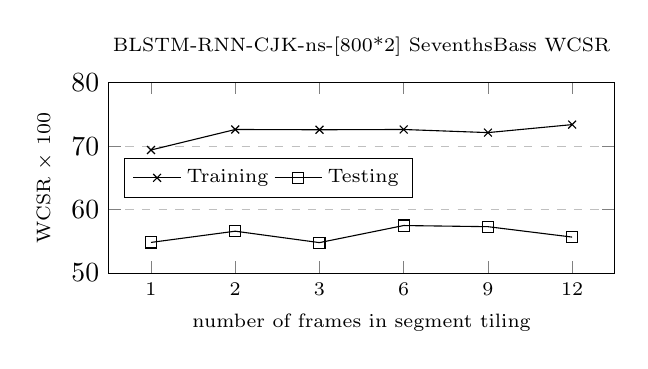
\begin{tikzpicture}
	\begin{axis}[
	title={BLSTM-RNN-CJK-ns-[800*2] SeventhsBass WCSR},
	title style = {font=\scriptsize},
	x label style={font=\scriptsize},
	symbolic x coords={1,2,3,6,9,12},
	x tick label style={font=\scriptsize},
	xtick=data,
	xlabel={number of frames in segment tiling},
	ylabel={WCSR $\times$ 100},
	y label style={font=\scriptsize},
	ymin=50, ymax=80,
	ytick={50,60,70,80},
	legend style={at={(0.03,0.5)},anchor=west,legend columns=-1, font=\scriptsize},
	ymajorgrids=true,
	grid style=dashed,
	]
	\addplot[ % Training
	color=black,
	mark=x,
	]
	coordinates {
		(1,69.39)(2,72.62)(3,72.58)(6,72.62)(9,72.13)(12,73.39)
	};
	
	\addplot[ % Testing
	color=black,
	mark=square,
	]
	coordinates {
		(1,54.83)(2,56.60)(3,54.80)(6,57.49)(9,57.31)(12,55.67)
	};
	\legend{Training, Testing} 
	\end{axis}
	\end{tikzpicture}
	\caption{Exploring effect of segment tiling. All systems are trained with CJK-ns-[800*2]}
	\label{fig:3-N-frame-ns}
\end{figure}

\Hsection{-ns level}
A set of systems are implemented using CJK-ns-[800*2] with different N-frame segment tiling. The experiment results are shown in Figure~\ref{fig:3-N-frame-ns}.

For MLP, it is clear that both training and testing score tends to decrease with the increase number of frames in segment tiling. This is odd at first sight, since normally with the increase of model complexity the training scores should also increase. But as mentioned before, since the training score is computed using the whole training+validation set, and as the MLP model is not strongly regularized as DBN does, therefore, if the increase of model complexity will downgrade testing performance, it also will downgrade the validation performance, and thus will slightly offset the training curve downwards. Based on this reasoning, the pattern here actually means the increase number of segment tiling frames tends to yield a worse model for MLP at -ns feature level.

For DBN, the plot shows that as the model complexity increases, the training score tends to increase and the testing score tends to decrease. The same conclusion as MLP's can be drawn from this pattern, that the increase number of segment tiling frames tends to yield a worse model for DBN at -ns feature level.

There is a good reason why both MLP and DBN peaks at $N=1$ in this case. They both try to look for order-irrelevant information, such as average pitch saliences to build up connections from input features to chord labels. A 1-frame segment tiling scheme is equal to representing each segment of chromagram by its time-averaged chroma, which simplifies the learning processes for both models. And the 1-frame segment tiling scheme actually introduces a strong (and incorrect) bias/assumption that the time order of pitches is irrelevant in classifying chords.

For BLSTM-RNN, while the training score increases, the testing score seems to peak at $N=6$. This on one hand indicates that segment tiling has a positive effect on BLSTM-RNN model, and on the other hand suggests that 6-frame might be a good choice in this case.

%\subsection{At -ch level, both MLP and DBN are impervious to training data size, while BLSTM-RNN benefits from more training data}\label{sec:3-p5}
\subsection{Training data size}\label{sec:3-p5}

\begin{figure}[htb]
	\centering
	\pgfplotsset{width=8cm,height=4cm,every node near coord/.append style={font=\scriptsize}}
	\subfigure{
		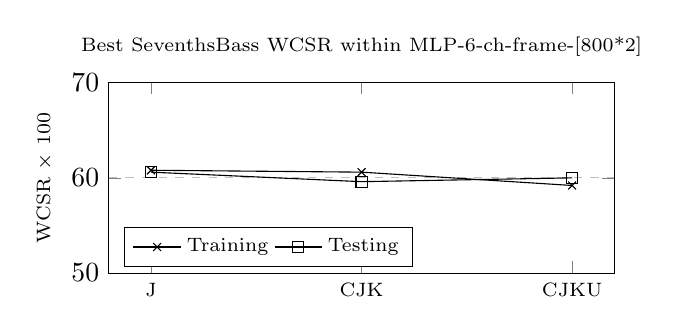
\begin{tikzpicture}
		\begin{axis}[
		title={Best SeventhsBass WCSR within MLP-6-ch-frame-[800*2]},
		title style = {font=\scriptsize},
		%xlabel={Network Configuration},
		x label style={font=\scriptsize},
		symbolic x coords={J,CJK,CJKU},
		x tick label style={font=\scriptsize},
		xtick=data,
		ylabel={WCSR $\times$ 100},
		y label style={font=\scriptsize},
		ymin=50, ymax=70,
		ytick={50,60,70},
		legend pos=south west,
		legend style={legend columns=-1, font=\scriptsize},
		ymajorgrids=true,
		grid style=dashed,
		]
		\addplot[ % Training
		color=black,
		mark=x,
		]
		coordinates {(J,60.8)(CJK,60.6)(CJKU,59.2)};
		
		\addplot[ % Testing
		color=black,
		mark=square,
		]
		coordinates {(J,60.6)(CJK,59.6)(CJKU,60.0)};
		\legend{Training, Testing} 
		\end{axis}
		\end{tikzpicture}
	}
	\subfigure{
		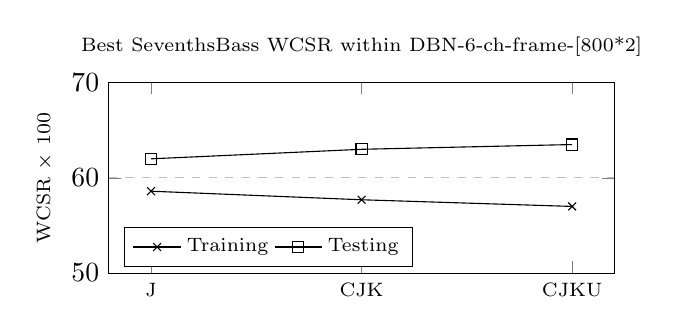
\begin{tikzpicture}
		\begin{axis}[
		title={Best SeventhsBass WCSR within DBN-6-ch-frame-[800*2]},
		title style = {font=\scriptsize},
		%xlabel={Network Configuration},
		x label style={font=\scriptsize},
		symbolic x coords={J,CJK,CJKU},
		x tick label style={font=\scriptsize},
		xtick=data,
		ylabel={WCSR $\times$ 100},
		y label style={font=\scriptsize},
		ymin=50, ymax=70,
		ytick={50,60,70},
		legend pos=south west,
		legend style={legend columns=-1, font=\scriptsize},
		ymajorgrids=true,
		grid style=dashed,
		]
		\addplot[ % Training
		color=black,
		mark=x,
		]
		coordinates {(J,58.6)(CJK,57.7)(CJKU,57.0)};
		
		\addplot[ % Testing
		color=black,
		mark=square,
		]
		coordinates {(J,62.0)(CJK,63.0)(CJKU,63.5)};
		\legend{Training, Testing} 
		\end{axis}
		\end{tikzpicture}
	}
	\subfigure{
		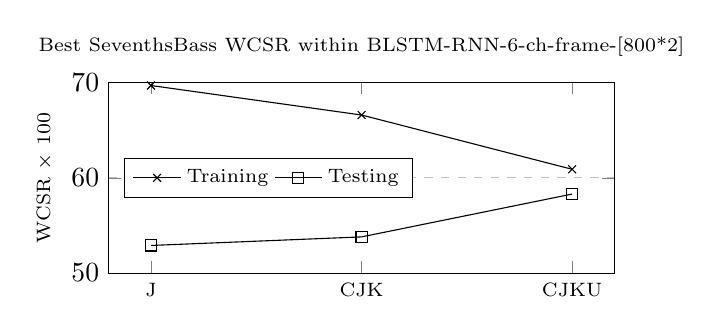
\begin{tikzpicture}
		\begin{axis}[
		title={Best SeventhsBass WCSR within BLSTM-RNN-6-ch-frame-[800*2]},
		title style = {font=\scriptsize},
		%xlabel={Network Configuration},
		x label style={font=\scriptsize},
		symbolic x coords={J,CJK,CJKU},
		x tick label style={font=\scriptsize},
		xtick=data,
		ylabel={WCSR $\times$ 100},
		y label style={font=\scriptsize},
		ymin=50, ymax=70,
		ytick={50,60,70},
		legend style={at={(0.03,0.5)},anchor=west,legend columns=-1, font=\scriptsize},
		ymajorgrids=true,
		grid style=dashed,
		]
		\addplot[ % Training
		color=black,
		mark=x,
		]
		coordinates {(J,69.7)(CJK,66.6)(CJKU,60.9)};
		
		\addplot[ % Testing
		color=black,
		mark=square,
		]
		coordinates {(J,52.9)(CJK,53.8)(CJKU,58.3)};
		\legend{Training, Testing} 
		\end{axis}
		\end{tikzpicture}
	}
	\caption{Exploring different training data size at -ch level. All systems are trained with 6-ch-frame-[800*2].}
	\label{fig:3-ch-data}
\end{figure}

\Hsection{-ch level}
Now the effect of training data size on different deep learning models will be examined. At -ch level, the results in Figure~\ref{fig:3-ch-data} show that both MLP and DBN are quite impervious to training data size, while BLSTM-RNN performs better with more data. 

For MLP and DBN, the results are consistent with all the previous results at -ch level. The dominating factor of the imperviousness here is the bass-treble chromagram feature itself. The prior imposed by this feature can be taken advantage of easily by the two models, and the amount of training data introduced cannot offset such high bias formed by the combination of the models and the feature.

For BLSTM-RNN, the results are also consistent with all previous results.With the increase of training data size, there are less variance in the model. In this model, the bias of bass-treble chromagram is not quite fully utilized as the other two models do.

Here is a plausible explanation as to why in Figure~\ref{fig:3-ch-data} (and Figure~\ref{fig:3-N-frame}) the testing scores of BLSTM-RNN are lower than the other two models. It is reasonable to think that BLSTM-RNN regards its input as a {\it sequence of frames}, while both MLP and DBN regard their inputs as \textit{2D images}. Therefore, while BLSTM-RNN tries to look for regularities within each pair of consecutive frames along the time direction, MLP and DBN could search regularities within every pair of frames along every possible directions. In many chord recognition cases, the latter approach is inevitably more efficient given that the input feature is already a very good summarization of pitch class saliences, but it also unavoidably suffers from the lack of consideration of ``sequential order'', which leads to over-fitting of root position chords, as will be demonstrated in Section~\ref{sec:3-p7}.


\begin{figure}[htb]
	\centering
	\pgfplotsset{width=8cm,height=4cm,every node near coord/.append style={font=\scriptsize}}
	\subfigure{
		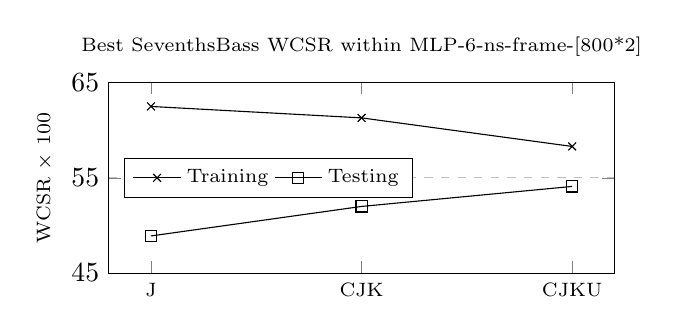
\begin{tikzpicture}
		\begin{axis}[
		title={Best SeventhsBass WCSR within MLP-6-ns-frame-[800*2]},
		title style = {font=\scriptsize},
		%xlabel={Network Configuration},
		x label style={font=\scriptsize},
		symbolic x coords={J,CJK,CJKU},
		x tick label style={font=\scriptsize},
		xtick=data,
		ylabel={WCSR $\times$ 100},
		y label style={font=\scriptsize},
		ymin=45, ymax=65,
		ytick={45,55,65},
		legend style={at={(0.03,0.5)},anchor=west,legend columns=-1, font=\scriptsize},
		ymajorgrids=true,
		grid style=dashed,
		]
		\addplot[ % Training
		color=black,
		mark=x,
		]
		coordinates {(J,62.5)(CJK,61.3)(CJKU,58.3)};
		
		\addplot[ % Testing
		color=black,
		mark=square,
		]
		coordinates {(J,48.9)(CJK,52.0)(CJKU,54.1)};
		\legend{Training, Testing} 
		\end{axis}
		\end{tikzpicture}
	}
	\subfigure{
		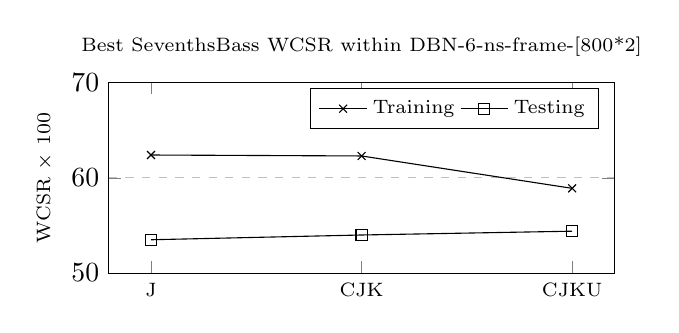
\begin{tikzpicture}
		\begin{axis}[
		title={Best SeventhsBass WCSR within DBN-6-ns-frame-[800*2]},
		title style = {font=\scriptsize},
		%xlabel={Network Configuration},
		x label style={font=\scriptsize},
		symbolic x coords={J,CJK,CJKU},
		x tick label style={font=\scriptsize},
		xtick=data,
		ylabel={WCSR $\times$ 100},
		y label style={font=\scriptsize},
		ymin=50, ymax=70,
		ytick={50,60,70},
		legend pos=north east,
		legend style={legend columns=-1, font=\scriptsize},
		ymajorgrids=true,
		grid style=dashed,
		]
		\addplot[ % Training
		color=black,
		mark=x,
		]
		coordinates {(J,62.4)(CJK,62.3)(CJKU,58.9)};
		
		\addplot[ % Testing
		color=black,
		mark=square,
		]
		coordinates {(J,53.5)(CJK,54.0)(CJKU,54.4)};
		\legend{Training, Testing} 
		\end{axis}
		\end{tikzpicture}
	}
	\subfigure{
		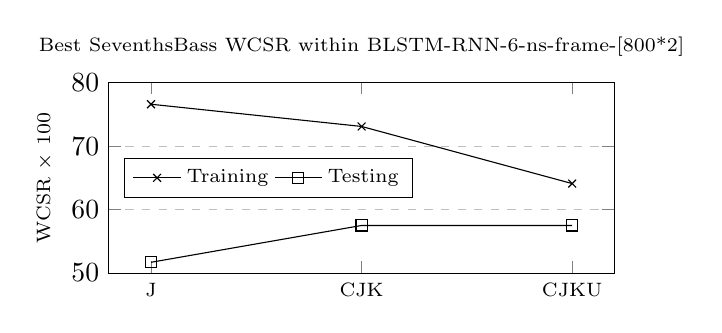
\begin{tikzpicture}
		\begin{axis}[
		title={Best SeventhsBass WCSR within BLSTM-RNN-6-ns-frame-[800*2]},
		title style = {font=\scriptsize},
		%xlabel={Network Configuration},
		x label style={font=\scriptsize},
		symbolic x coords={J,CJK,CJKU},
		x tick label style={font=\scriptsize},
		xtick=data,
		ylabel={WCSR $\times$ 100},
		y label style={font=\scriptsize},
		ymin=50, ymax=80,
		ytick={50,60,70,80},
		legend style={at={(0.03,0.5)},anchor=west,legend columns=-1, font=\scriptsize},
		ymajorgrids=true,
		grid style=dashed,
		]
		\addplot[ % Training
		color=black,
		mark=x,
		]
		coordinates {(J,76.6)(CJK,73.1)(CJKU,64.1)};
		
		\addplot[ % Testing
		color=black,
		mark=square,
		]
		coordinates {(J,51.7)(CJK,57.5)(CJKU,57.5)};
		\legend{Training, Testing} 
		\end{axis}
		\end{tikzpicture}
	}
	\subfigure{
		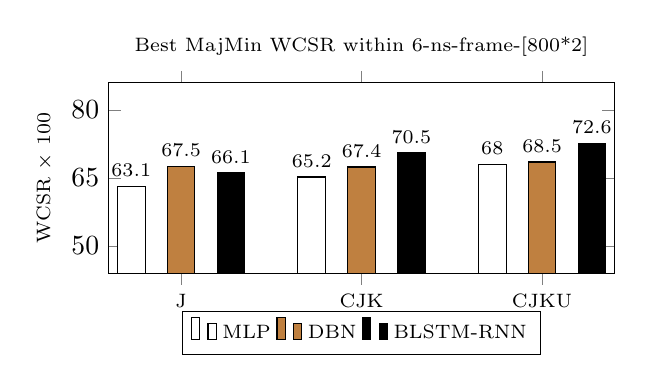
\begin{tikzpicture}
		\begin{axis}[
		title={Best MajMin WCSR within 6-ns-frame-[800*2]},
		title style = {font=\scriptsize},
		ybar=8pt,
		enlargelimits=0.2,
		legend style={at={(0.5,-0.2)},
			anchor=north,legend columns=-1},
		ylabel={WCSR $\times$ 100},
		y label style={font=\scriptsize},
		symbolic x coords={J,CJK,CJKU},
		x tick label style={font=\scriptsize},
		xtick=data,
		ymin=50, ymax=80,
		ytick={50,65,80},
		nodes near coords,
		nodes near coords align={vertical},
		legend style={font=\scriptsize},
		]
		\addplot [ybar,fill=white,draw=black] coordinates {(J,63.1)(CJK,65.2)(CJKU,68.0)};
		\addplot [ybar,fill=brown,draw=black] coordinates {(J,67.5)(CJK,67.4)(CJKU,68.5)};
		\addplot [ybar,fill=black,draw=black] coordinates {(J,66.1)(CJK,70.5)(CJKU,72.6)};
		\legend{MLP,DBN,BLSTM-RNN}
		\end{axis}
		\end{tikzpicture}
	}
	\caption{Exploring training data size at -ns level. All systems are trained with 6-ns-frame-[800*2].}
	\label{fig:3-ns-data}
\end{figure}

\Hsection{-ns level}
At -ns level, as shown in Figure~\ref{fig:3-ns-data}, with more training data, DBN still exhibits similar imperviousness in testing score with less variance, while both MLP and BLSTM-RNN have better testing scores and less variance with larger data size. In the case of DBN, this means the network might be over-regularized in the pre-training process, but nevertheless, the model's variance decrease with the increase of training data. As for MLP, since it is not so strongly regularized, it not only has less variance, but also better generalization ability as the training set grows.

BLSTM-RNN behaves similarly as MLP does, but interestingly, although it does not show any SeventhsBass improvement from CJK to CJKU, the improvement happens in MajMin (see the last subfigure of Figure~\ref{fig:3-ns-data}), albeit MajMin is not a direct training objective. In Section~\ref{sec:3-p8} we will see that this actually means it tends to make mistakes/confusions in a more acceptable way.

At -ns level, there is no strong prior such as bass-treble chromagram being introduced, so that it almost all depends on the fitness of a model to learn meaningful regularities from the data. The above results illustrate that as the training data size grows, BLSTM-RNN model tends to have better generalization ability than the other two models, and it tends to make more acceptable labeling confusions. As discussed before, BLSTM-RNN employs an order-relevant approach in learning. The tuned notegram at -ns level maintains important raw information about ``order'', such as pitch continuity, voicing, bass positions and bass ordering, which helps BLSTM-RNN learn a good model. On the other hand, while MLP and DBN are regarding the -ns features as 2D images, it is more difficult to retrieve chord-related regularities compared with the -ch features.

%\subsection{BLSTM-RNN recognizes long-tail chords well, while MLP and DBN tend to over-fit common chords}\label{sec:3-p7}
\subsection{Skewed classes}\label{sec:3-p7}

\begin{figure*}[htb]
	\centering
	\pgfplotsset{width=18cm,height=4cm,every node near coord/.append style={font=\scriptsize}}
	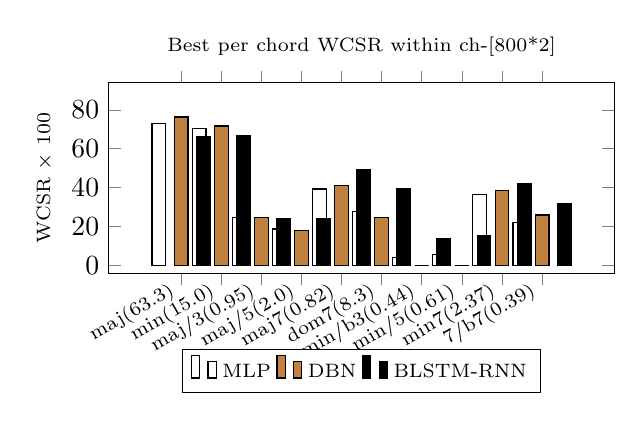
\begin{tikzpicture}
	\begin{axis}[
	title={Best per chord WCSR within ch-[800*2]},
	title style = {font=\scriptsize},
	ybar=3pt,
	bar width=5pt,
	enlargelimits=0.2,
	legend style={at={(0.5,-0.4)},
		anchor=north,legend columns=-1},
	ylabel={WCSR $\times$ 100},
	y label style={font=\scriptsize},
	symbolic x coords={maj(63.3), min(15.0), maj/3(0.95), maj/5(2.0), maj7(0.82), dom7(8.3), min/b3(0.44), min/5(0.61), min7(2.37), 7/b7(0.39)},
	x tick label style={rotate=30,anchor=east, font=\scriptsize},
	xtick=data,
	ymin=10, ymax=80,
	%nodes near coords,
	nodes near coords align={vertical},
	legend style={font=\scriptsize},
	]
	\addplot [ybar,fill=white,draw=black] coordinates {(maj(63.3),73.1)(min(15.0),70.3)(maj/3(0.95),24.7)(maj/5(2.0),18.7)(maj7(0.82),39.3)(dom7(8.3),27.8)(min/b3(0.44),4.2)(min/5(0.61),5.4)(min7(2.37),36.6)(7/b7(0.39),22.2)};
	
	\addplot [ybar,fill=brown,draw=black] coordinates {(maj(63.3),76.3)(min(15.0),71.7)(maj/3(0.95),24.6)(maj/5(2.0),18.1)(maj7(0.82),41.3)(dom7(8.3),24.7)(min/b3(0.44),0)(min/5(0.61),0)(min7(2.37),38.3)(7/b7(0.39),25.9)};
	
	\addplot [ybar,fill=black,draw=black] coordinates {(maj(63.3),66.2)(min(15.0),66.6)(maj/3(0.95),24.0)(maj/5(2.0),24.3)(maj7(0.82),49.1)(dom7(8.3),39.7)(min/b3(0.44),13.9)(min/5(0.61),15.4)(min7(2.37),42.2)(7/b7(0.39),32.0)};
	
	\legend{MLP,DBN,BLSTM-RNN}
	\end{axis}
	\end{tikzpicture}
	\caption{Different models' handling of uncommon and common chords. All systems are trained with ch-[800*2]. Numbers in brackets indicates the percentage of chord within the test set.}
	\label{fig:3-blstm-long-tail}
\end{figure*}
A detail investigation of performances on skewed classes reveals the true potential of BLSTM-RNN that makes us believe it to be a better model at handling large vocabulary ACE in a pre-segmentation framework. In short: 1) BLSTM-RNN performs much better than MLP and DBN on uncommon chords (i.e., chords with minority population), while both MLP and DBN tend to over-fit common chords (i.e., chords with major population); 2) BLSTM-RNN scores much better in a balanced performance metric.
%BLSTM-RNN makes balanced and steady progress in all categories with the increase of training data.

Figure~\ref{fig:3-blstm-long-tail} shows how different models perform on different chords (or ``chord types'', used interchangeably with ``chords'' in this context). These performances are reported as per chord WCSR:
\begin{equation}
	\mathit{WCSR_{chord} = {\sum{Length(chord_i)*CSR_i} \over \sum{Length(chord_i)}}},
	\label{eq:3-wcsrchord}
\end{equation}
where the subscript $i$ denotes the $i^{th}$ instance of the chord within the data set. Among all chord types, \textit{maj} and \textit{min} are unarguably considered common chords, because they constitute the major population in pop/rock music practice \cite{burgoyne2011expert}, and specifically in both the training and testing sets. The other chords are considered uncommon. As demonstrated, the main advantage of MLP and DBN over BLSTM-RNN appears in \textit{maj} and \textit{min}, but BLSTM-RNN outperforms the two other models by large amounts in most uncommon chords. Note that based on Equation~\ref{eq:3-csr} and~\ref{eq:3-wcsr}, even small advantages in common chords could eventually lead to large advantages in overall \textit{WCSR}s.

\begin{figure}[htb]
	\centering
	\pgfplotsset{width=6cm,height=4cm,every node near coord/.append style={font=\scriptsize}}
	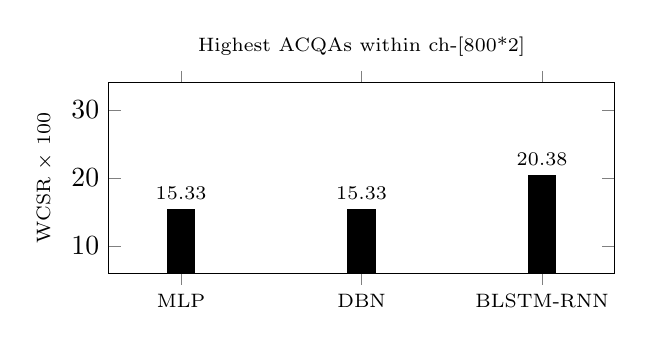
\begin{tikzpicture}
	\begin{axis}[
	title={Highest ACQAs within ch-[800*2]},
	title style = {font=\scriptsize},
	ybar=8pt,
	enlargelimits=0.2,
	legend style={at={(0.5,-0.2)},
		anchor=north,legend columns=-1},
	ylabel={WCSR $\times$ 100},
	y label style={font=\scriptsize},
	symbolic x coords={MLP,DBN,BLSTM-RNN},
	x tick label style={font=\scriptsize},
	xtick=data,
	ymin=10, ymax=30,
	nodes near coords,
	nodes near coords align={vertical},
	legend style={font=\scriptsize},
	]
	%\addplot [ybar,fill=black,draw=black] coordinates {(MLP,291.21)(DBN,291.23)(BLSTM-RNN,387.2)};
	\addplot [ybar,fill=black,draw=black] coordinates {(MLP,15.33)(DBN,15.33)(BLSTM-RNN,20.38)};
	\end{axis}
	\end{tikzpicture}
	\caption{ACQAs in all SeventhsBass Chord Categories. All systems are trained with ch-[800*2].}
	\label{fig:3-sumofsb}
\end{figure}

To measure well-roundedness of a model, ``Average Chord Quality Accuracy''(\textit{ACQA}) index \cite{cho2014improved} is used. It averages the \textit{WCSR}s of all chord types in the test vocabulary without weighting:
\begin{equation}
	\mathit{ACQA = {{\sum{WCSR_{chord}}} \over {\#\,of\,chords}}}.
	\label{eq:3-acqa}
\end{equation}
Alternatively, a \textit{CQA} would stand for ``Chord Quality Accuracy'':
\begin{equation}
\mathit{CQA = \sum{WCSR_{chord}}}.
\label{eq:3-cqa}
\end{equation}
Models that over-fit on a few chord types tend to get lower \textit{ACQA}s, while those well balanced systems will have higher \textit{ACQA}s. As shown in Figure~\ref{fig:3-sumofsb}, the highest \textit{ACQA} of BLSTM-RNNs outscores the highest of the other two by around five points. This well demonstrates that BLSTM-RNN generalizes much better. Referring back to Section~\ref{sec:3-p5}, this also indicates that both MLP and DBN over-fit the common chords.

\subsection{Confusions and tolerations} \label{sec:3-p8}

\begin{figure}[htb]
	\centering
	\includegraphics[width=1\columnwidth,height=0.6\columnwidth]{3/figures/ds-eps-converted-to.pdf}
	\caption{Boxplot of the score differences of different vocabulary (for all system variants considered in this paper). Mm = MajMin; MmB = MajMinBass; S = Sevenths; SB = SeventhsBass}
	\label{fig:3-ds}
\end{figure}

In the above discussions, there are mainly SeventhsBass results. However, in the MIREX ACE evaluation, three other vocabularies are evaluated, namely, MajMin, Maj-MinBass, and Sevenths (already introduced in Section~\ref{sec:3-aceeval}). Their scores are calculated based on SeventhsBass with certain toleration of two types of chord confusions:
\begin{itemize}
	\item Bass confusion, where the estimation has the same root and quality as the reference, but has a different bass (e.g., confusion between root position and inversion);
	\item Seventh confusion, where the estimation has the same root and bass as the reference, but has a different quality with regard to the seventh type (e.g., confusion between maj and maj7, between 7 and maj7, or between min/b3 and min7/b3).
\end{itemize}

With these definitions, the other three vocabularies' scores can be interpreted as follows. Upon the SeventhsBass score:
\begin{itemize}
	\item Sevenths tolerates all bass confusions;
	\item MajMinBass tolerates all seventh confusion; and
	\item MajMin tolerates both.
\end{itemize}
The rationale behind these tolerations is that if such confusions happen, the difference of the original harmony and the new/modified harmony may still be within an acceptable range. Another perspective to understand this would be that human will sometimes also make these confusions.
%By clarifying that, SeventhsBass is the strictest evaluation among all; Sevenths and MajMinBass are less strict, both with relaxation of one confusion type; MajMin is the loosest, with both types tolerated.

% ** according to R2, not necessary to show both figures
Figure~\ref{fig:3-ds} is a boxplot showing the amount of these confusions/tolerations for all system variants implemented in this paper. In the plot, the amount of bass confusions (S-SB) is very focused around 2, while the other two differences are also focused with less than 2.5 between the first and third quartiles.

\subsection{Baseline Comparison} \label{sec:3-p9}

\begin{figure}[htb]
	\centering
	\pgfplotsset{width=9cm,height=5cm,every node near coord/.append style={font=\tiny}}
	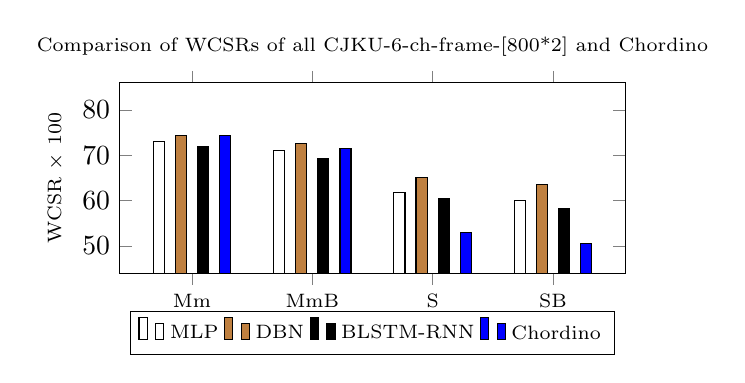
\begin{tikzpicture}
	\begin{axis}[
	title={Comparison of WCSRs of all CJKU-6-ch-frame-[800*2] and Chordino},
	title style = {font=\scriptsize},
	ybar=4pt,
	bar width=4pt,
	enlargelimits=0.2,
	legend style={at={(0.5,-0.2)},
		anchor=north,legend columns=-1},
	ylabel={WCSR $\times$ 100},
	y label style={font=\scriptsize},
	symbolic x coords={Mm,MmB,S,SB},
	x tick label style={font=\scriptsize},
	xtick=data,
	ymin=50, ymax=80,
	%nodes near coords,
	%nodes near coords align={vertical},
	legend style={font=\scriptsize},
	]
	\addplot [ybar,fill=white,draw=black] coordinates {(Mm,73.1)(MmB,71.0)(S,61.87)(SB,60.04)};
	
	\addplot [ybar,fill=brown,draw=black] coordinates {(Mm,74.35)(MmB,72.5)(S,65.1)(SB,63.5)};
	
	\addplot [ybar,fill=black,draw=black] coordinates {(Mm,72.0)(MmB,69.2)(S,60.5)(SB,58.3)};
	
	\addplot [ybar,fill=blue,draw=black] coordinates {(Mm,74.3)(MmB,71.4)(S,53.0)(SB,50.6)};
	
	\legend{MLP, DBN, BLSTM-RNN, Chordino}
	\end{axis}
	\end{tikzpicture}
	\caption{Compare with Chordino - MIREX metrics. All systems are trained with CJKU-6-ch-frame-[800*2]. Mm = MajMin; MmB = MajMinBass; S = Sevenths; SB = SeventhsBass}
	\label{fig:3-compchordino}
\end{figure}

\begin{figure}[htb]
	\centering
	\pgfplotsset{width=8cm,height=4cm,every node near coord/.append style={font=\scriptsize}}
	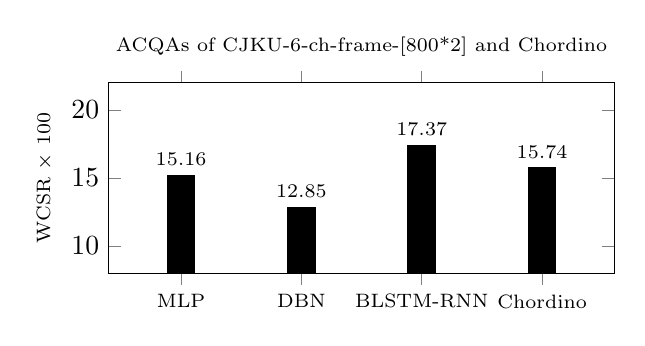
\begin{tikzpicture}
	\begin{axis}[
	title={ACQAs of CJKU-6-ch-frame-[800*2] and Chordino},
	title style = {font=\scriptsize},
	ybar=8pt,
	enlargelimits=0.2,
	legend style={at={(0.5,-0.2)},
		anchor=north,legend columns=-1},
	ylabel={WCSR $\times$ 100},
	y label style={font=\scriptsize},
	symbolic x coords={MLP,DBN,BLSTM-RNN,Chordino},
	x tick label style={font=\scriptsize},
	xtick=data,
	ymin=10, ymax=20,
	nodes near coords,
	nodes near coords align={vertical},
	legend style={font=\scriptsize},
	]
	%\addplot [ybar,fill=black,draw=black] coordinates {(MLP,288.1)(DBN,244.1)(BLSTM-RNN,330.1)(Chordino,299.0)};
	\addplot [ybar,fill=black,draw=black] coordinates {(MLP,15.16)(DBN,12.85)(BLSTM-RNN,17.37)(Chordino,15.74)};
	\end{axis}
	\end{tikzpicture}
	\caption{Comparison of ACQAs of CJKU-6-ch-frame-[800*2] and Chordino}
	\label{fig:3-acqachordino}
\end{figure}

At last some best system representatives are compared with the baseline approach - Chordino. There is one representative for each deep learning model, all trained with CJKU-6-ch-frame-[800*2]. They are compared with Chordino in terms of five categories: four \textit{WCSR}s (Figure~\ref{fig:3-compchordino}) and the \textit{ACQA} (Figure~\ref{fig:3-acqachordino}).

As shown, these systems all outperform Chordino by a large amount in S and SB, and they are fairly comparable with Chordino in Mm and MmB. In terms of versatility, Chordino is not bad at all, outperforming both MLPs and DBN's representatives, but obviously the most balanced system is based on BLSTM-RNN.

\section{MIREX 2016 Results}
MIREX ACE 2016 features 4 sets of systems implemented by four different groups:
\begin{itemize}
\item CM1: Chordino, from Queen Mary University of London;
\item DK*: features three variants of the ACE approach proposed in this chapter (note that DK4, which is from another design approach, is skipped in the following discussion);
\item FK*: implemented by Korzeniowski and Widmer, featuring the systems in two previous papers \cite{Korzeniowski2016feature,Korzeniowski2016convolutional}
\item KO1: shineChords, a time-frequency reassign approach proposed by Khadkevich and Omologo \cite{khadkevich2011time}.
\end{itemize}

\subsection{Dataset and Vocabulary}
It should be noted that except CM3, whose model parameters are all manually specified, all other systems involve extensive training:
\begin{itemize}
\item KO1's description does not mention its training set, but it is probably trained with the Isophonic dataset (MIREX 2009 set) \cite{burgoyne2014comparative}. This can be easily spot by simply noticing that, compared with other systems, it has too high a SB score in Isophonic, while not as high in other test sets.

\item FK* are trained with the Isophonic, Robbie Williams \footnote{\url{https://www.researchgate.net/publication/260399240\_Chord\_and\_Harmony\_annotations\_of\_the\_first\_five\_albums\_by\_Robbie\_Williams}}, RWC and the public part of McGill Billboard \footnote{\url{http://ddmal.music.mcgill.ca/billboard}} dataset.

\item DK* are trained with USPop and RWC dataset. Note that they do not contain any test set in MIREX ACE 2016.
\end{itemize}

In terms of chord vocabulary, both DK3, FK* and KO1 only support majmin, CM1 supports a large vocabulary including most types in SeventhsBass, and DK1\&2 support exactly the SeventhsBass.

\begin{table*}[htb]
\centering
\scriptsize
\caption{MIREX 2016 Results}
\label{tab:3-mirex2016}
\begin{tabular}{|c|c|c|c|c|c|c|c|c|}\hline
Algorithm & R & Mm & MmB & S & SB & Seg & UnderSeg & OverSeg \\ \hline
Isophonics 2009\\ \hline
CM1 & 78.56 & 75.41 & 72.48 & 54.67 & 52.26 & 85.90 & 87.17 & 86.09\\ \hline
DK1 & 79.21 & 76.19 & 74.00 & 66.02 & 64.15 & 85.71 & 82.62 & 91.23\\ \hline
DK2 & 77.84 & 74.49 & 71.93 & 61.61 & 59.47 & 85.82 & 82.72 & 91.28\\ \hline
DK3 & 80.03 & 77.55 & 74.79 & 68.40 & 65.88 & 85.81 & 82.50 & 91.53\\ \hline
DK4 & 76.05 & 72.96 & 71.41 & 62.77 & 61.44 & 78.19 & 87.97 & 72.43\\ \hline
FK2 & 86.09 & 85.53 & 82.24 & 74.42 & 71.54 & 87.76 & 85.79 & 90.73\\ \hline
FK4 & 82.28 & 80.93 & 78.03 & 70.91 & 68.26 & 85.62 & 82.40 & 90.89\\ \hline
KO1 & 82.93 & 82.19 & 79.61 & 76.04 & 73.43 & 87.69 & 85.66 & 91.24\\ \hline
Billboard 2012 \\ \hline
CM1 & 74.15 & 72.22 & 70.21 & 55.35 & 53.40 & 83.64 & 85.31 & 83.39\\ \hline
DK1 & 75.28 & 73.57 & 71.87 & 59.98 & 58.53 & 83.35 & 80.26 & 88.52\\ \hline
DK2 & 73.77 & 71.69 & 69.86 & 58.66 & 57.00 & 83.57 & 80.40 & 88.70\\ \hline
DK3 & 75.92 & 74.75 & 72.69 & 53.42 & 51.67 & 83.39 & 79.97 & 88.92\\ \hline
DK4 & 72.59 & 70.85 & 69.78 & 56.29 & 55.36 & 76.13 & 87.72 & 70.05\\ \hline
FK2 & 85.64 & 85.38 & 82.55 & 60.70 & 58.38 & 87.62 & 86.09 & 90.13\\ \hline
FK4 & 79.23 & 78.62 & 76.20 & 56.53 & 54.51 & 85.09 & 81.98 & 89.94\\ \hline
KO1 & 77.45 & 75.58 & 73.51 & 57.68 & 55.82 & 84.16 & 82.80 & 87.44\\ \hline
Billboard 2013 \\ \hline
CM1 & 71.16 & 67.28 & 65.20 & 48.99 & 47.17 & 81.54 & 83.11 & 82.63\\ \hline
DK1 & 72.06 & 68.69 & 67.26 & 54.54 & 53.29 & 80.82 & 77.58 & 88.06\\ \hline
DK2 & 70.18 & 66.54 & 64.66 & 52.97 & 51.41 & 80.85 & 77.68 & 88.02\\ \hline
DK3 & 72.39 & 68.53 & 66.55 & 48.99 & 47.28 & 80.76 & 77.26 & 88.30\\ \hline
DK4 & 69.56 & 65.83 & 64.78 & 51.81 & 50.93 & 74.55 & 86.31 & 69.18\\ \hline
FK2 & 80.07 & 77.89 & 75.42 & 55.41 & 53.22 & 82.94 & 82.43 & 86.80\\ \hline
FK4 & 74.66 & 71.85 & 69.44 & 51.93 & 49.80 & 80.61 & 77.19 & 88.70\\ \hline
KO1 & 75.36 & 71.39 & 69.43 & 53.57 & 51.78 & 81.63 & 79.61 & 87.75\\ \hline
JayChou 2015 \\ \hline
CM1 & 72.75 & 72.08 & 65.48 & 54.39 & 48.98 & 86.60 & 86.89 & 86.91\\ \hline
DK1 & 74.70 & 73.87 & 70.33 & 54.98 & 52.25 & 86.76 & 82.78 & 91.79\\ \hline
DK2 & 72.19 & 72.55 & 69.10 & 54.09 & 51.46 & 87.09 & 83.35 & 91.75\\ \hline
DK3 & 75.01 & 74.75 & 63.56 & 49.27 & 40.24 & 86.76 & 82.54 & 92.08\\ \hline
DK4 & 71.51 & 69.03 & 65.93 & 50.07 & 47.45 & 78.11 & 87.87 & 70.56\\ \hline
FK2 & 79.51 & 78.66 & 68.15 & 50.69 & 42.34 & 86.81 & 85.43 & 88.56\\ \hline
FK4 & 76.13 & 75.44 & 64.36 & 49.69 & 40.74 & 84.55 & 81.22 & 88.95\\ \hline
KO1 & 78.73 & 77.69 & 66.87 & 54.16 & 44.55 & 88.46 & 87.12 & 90.11\\ \hline
RobbieWilliams 2016 \\ \hline
CM1 & 81.90 & 78.25 & 76.05 & 57.92 & 55.90 & 87.96 & 88.96 & 87.45\\ \hline
DK1 & 81.50 & 77.77 & 76.10 & 68.88 & 67.34 & 87.03 & 83.22 & 92.11\\ \hline
DK2 & 79.01 & 75.97 & 73.57 & 65.26 & 62.98 & 87.20 & 83.40 & 92.23\\ \hline
DK3 & 81.85 & 78.56 & 76.16 & 74.71 & 72.55 & 86.98 & 82.95 & 92.34\\ \hline
DK4 & 78.92 & 75.15 & 73.66 & 66.72 & 65.34 & 81.82 & 88.44 & 76.88\\ \hline
FK2 & 88.53 & 87.23 & 84.19 & 82.57 & 79.88 & 90.04 & 88.62 & 91.88\\ \hline
FK4 & 83.37 & 80.96 & 78.42 & 77.04 & 74.76 & 87.22 & 84.50 & 91.02\\ \hline
KO1 & 83.55 & 80.33 & 78.16 & 73.54 & 71.39 & 88.04 & 85.39 & 91.68\\ \hline
\end{tabular}
\end{table*}
\subsection{Results and Discussions}
Table~\ref{tab:3-mirex2016} shows the results of MIREX ACE 2016 \footnote{B = Bass, Mm = MajMin, MmB = MajMinBass, R = Root, S = Sevenths, SB = SeventhsBass, Seg = Segmentation Quality}. Within the context of this thesis, the main focus of the results is the SeventhsBass column.

In Isophonic test, KO1 gets the highest score. But this is probably because of its over-fitting the data, as explained previously, that it actually scores much lower in tests that it does not previously know, such as JayChou 2015. Both FK2 and FK4 come next to KO1, but unfortunately they are all informed with this test set. Since it is not clear to what extend the systems over-learn the data, the results of this test is not statistically valid to deduce any reasonable conclusions regarding these systems.

In Billboard 2012 and 2013 tests, the best performances are both from DK1. Although FK* learn from part of the test set, they somehow does not outperform DK1. Moreover, DK1 outscore KO1 by about 3 points in both tests, which demonstrates a better generalization capability in DK1 system.

JayChou 2015 test is probably the most convincing one, since on one had none of the systems are learning this set, and on the other hand it has more than 20\% of chords other than maj, min and sevenths, much more than other test sets. The performance on this test could well demonstrate the system's vocabulary versatility. This can be noticed by making comparison within the DK* systems, where DK1 and DK2 perform much better than DK3 in SB. The best two systems in this test are DK1 and DK2, outscoring the FK* systems by around 10 points, and the KO1 system by about 8 points.

Robbie Williams test somehow shows the reverse ranking of JayChou 2015. DK3 leads both DK1 and DK2 by about 5 and 10 points. FK* are the best performing ones, but unfortunately they might over-learn the data. It is interesting to note that KO1 scores 71.39, slightly less that DK3's 72.55. This strongly indicates that this test is mainly composed of maj, min and sevenths (probably > 90\%), which is very similar to the chord composition of the Isophonic set. Therefore systems that only support a small chord vocabulary will have a huge advantage by not being able to have confusions on long-tail chords.

\section{On Smaller Vocabulary}
This chapter is mainly developed based on large vocabulary, specifically, the SeventhsBass vocabulary. In order to do a comparison between the proposed system framework and other approaches, a set of experiments are conducted using two smaller vocabularies: 1, MajMin; 2, Full121 vocabulary introduced by Mauch \cite{mauch2010automatic} (also mentioned in Section~\ref{sec:3-2-largevocab}). For MajMin system implementation, each label in the training set will be mapped to its MajMin form following a normal mapping scheme \cite{harte2010towards,pauwels2013evaluating}. As a result, each deep learning model will be trained on a dataset with only MajMin labels. For Full121 implementation, a slightly modified version of chord mapping strategy \cite{mauch2010automatic} is followed.

\subsection{On MajMin}
Table~\ref{tab:3-overallres} shows a SeventhsBass evaluation comparison, where all systems, except for Chordino, only supports MajMin vocabulary. The results show that on one hand the overall performances of these systems are only fairly comparable with those in Section~\ref{sec:3-p9}, on the other hand the CQA of these systems are all much lower because of a much smaller vocabulary than Chordino.
\begin{table}[h]
\footnotesize
\centering
\caption{Overall WCSR scores; All systems are trained with CJKUR-(800,800), with only MajMin vocabulary support.}
\label{tab:3-overallres}
\begin{tabular}{|c|c|c|c|c|c|c|c|c|}\hline
System & B & Mm & MmB & R & S & SB & Seg & CQA \\ \hline
chordino & 76.41 & 74.30 & 71.40 & 77.19 & 52.99 & 50.60 & 83.87 & 299.01\\ \hline
MLP-ch & 74.71 & 73.25 & 71.22 & 75.74 & 65.08 & 63.18 & 83.57 & 151.57\\ \hline
DBN-ch & 77.04 & 75.50 & 73.39 & 78.10 & 67.26 & 65.30 & 83.78 & 156.80\\ \hline
BLSTM-RNN-ch & 76.88 & 75.05 & 72.84 & 78.11 & 66.58 & 64.50 & 83.74 & 157.46\\ \hline
MLP-ns & 72.65 & 70.00 & 68.14 & 73.35 & 62.72 & 60.98 & 83.59 & 140.57\\ \hline
DBN-ns & 72.91 & 70.96 & 69.14 & 73.66 & 63.33 & 61.66 & 83.44 & 144.89\\ \hline
BLSTM-RNN-ns & 76.04 & 73.98 & 71.99 & 76.85 & 65.85 & 64.03 & 83.76 & 153.63\\ \hline
\end{tabular}
\end{table}

Table~\ref{tab:3-detailres} shows the SeventhsBass categorical breakdown. Take DBN-ch as representative, since it only supports MajMin, its $maj$ and $min$ scores are much higher than the Chordino's. As the two chord types comprise of the majority of the data set population, that's why it has a much higher SB score. However, by relaxing the evaluation strength from SB to Mm, the performance difference between DBN-ch and Chordino becomes less and less.

\begin{landscape}
\thispagestyle{plain}
\begin{table*}[h]
\scriptsize
\caption{Detail SeventhsBass WCSR scores. All systems are trained with CJKUR-(800,800), with only MajMin vocabulary support. M = Major, m = minor, N = no chord. The \%B row shows the composition of chords in the test dataset.}
\label{tab:3-detailres}
\begin{tabular}{|c|c|c|c|c|c|c|c|c|c|c|c|c|c|c|c|c|c|c|c|}\hline
\%B & 2.01 & 0.95 & 63.31 & 0.02 & 0.17 & 0.27 & 0.82 & 0.08 & 0.06 & 0.39 & 8.33 & 0.61 & 0.44 & 14.99 & 0.01 & 0.06 & 0.41 & 2.37 & 4.63\\ \hline
 & M/5 & M/3 & M & M7/5 & M7/3 & M7/7 & M7 & 7/5 & 7/3 & 7/b7 & 7 & m/5 & m/b3 & m & m7/5 & m7/b3 & m7/b7 & m7 & N\\ \hline
chordino & 19.9 & 17.1 & 54.4 & 0.0 & 0.0 & 0.0 & 55.6 & 0.0 & 0.0 & 5.7 & 41.0 & 0.0 & 0.0 & 54.3 & 0.0 & 0.0 & 0.0 & 51.0 & 2.2\\ \hline
MLP-ch & 0.0 & 0.0 & 77.6 & 0.0 & 0.0 & 0.0 & 0.0 & 0.0 & 0.0 & 0.0 & 0.0 & 0.0 & 0.0 & 74.0 & 0.0 & 0.0 & 0.0 & 0.0 & 2.8\\ \hline
DBN-ch & 0.0 & 0.0 & 80.0 & 0.0 & 0.0 & 0.0 & 0.0 & 0.0 & 0.0 & 0.0 & 0.0 & 0.0 & 0.0 & 76.8 & 0.0 & 0.0 & 0.0 & 0.0 & 3.0\\ \hline
BLSTM-RNN-ch & 0.0 & 0.0 & 79.3 & 0.0 & 0.0 & 0.0 & 0.0 & 0.0 & 0.0 & 0.0 & 0.0 & 0.0 & 0.0 & 78.2 & 0.0 & 0.0 & 0.0 & 0.0 & 2.5\\ \hline
MLP-ns & 0.0 & 0.0 & 76.4 & 0.0 & 0.0 & 0.0 & 0.0 & 0.0 & 0.0 & 0.0 & 0.0 & 0.0 & 0.0 & 64.2 & 0.0 & 0.0 & 0.0 & 0.0 & 2.9\\ \hline
DBN-ns & 0.0 & 0.0 & 76.3 & 0.0 & 0.0 & 0.0 & 0.0 & 0.0 & 0.0 & 0.0 & 0.0 & 0.0 & 0.0 & 68.6 & 0.0 & 0.0 & 0.0 & 0.0 & 2.9\\ \hline
BLSTM-RNN-ns & 0.0 & 0.0 & 79.0 & 0.0 & 0.0 & 0.0 & 0.0 & 0.0 & 0.0 & 0.0 & 0.0 & 0.0 & 0.0 & 74.7 & 0.0 & 0.0 & 0.0 & 0.0 & 2.7\\ \hline
\end{tabular}
\end{table*}
\end{landscape}

\subsection{On Full121}

\begin{table}[h]
\footnotesize
\centering
\caption{Full121 WCSR scores. Tested on TheBeatles180 dataset (180 tracks out of the 216 tracks Isophonic 2009) All systems are trained with CJKUR-(800,800)-ch, with Full121 vocabulary support.}
\label{tab:3-full}
\begin{tabular}{|c|c|c|}\hline
System & Full121 WCSR & Seg \\ \hline
MLP & 73.43 & 83.77 \\ \hline
DBN & 75.46 & 83.92 \\ \hline
BLSTM-RNN & 73.63 & 83.80 \\ \hline
\end{tabular}
\end{table}

\begin{table}[h]
\footnotesize
\centering
\caption{Full121 scores. Tested on Isophonic 2009 dataset with 3-fold cross-validation\cite{ni2012end}}
\label{tab:3-fullhp}
\begin{tabular}{|c|c|c|}\hline
System & Full121 Chord Precision (CP) & Seg \\ \hline
CH(Chordino) & 50.31 & N/A \\ \hline
HP(Harmonic Analyzer) & 70.26 & N/A\\ \hline
\end{tabular}
\end{table}

\begin{table}[h]
\footnotesize
\centering
\caption{Full121 scores. Tested on Isophonic 2009 dataset with 5-fold cross-validation \cite{mauch2010automatic}}
\label{tab:3-fullmbk}
\begin{tabular}{|c|c|c|}\hline
System & Full121 Relative Correct Overlap (RCO) & Seg \\ \hline
trained MBK & 41.8 & N/A \\ \hline
MBK & 56.7 & 77.9 \\ \hline
MBK-NNLS & 61.8 & N/A \\ \hline
\end{tabular}
\end{table}

Table~\ref{tab:3-full} shows results of Full121 vocabulary with the same test set. Table~\ref{tab:3-fullhp} and ~\ref{tab:3-fullmbk} shows Full121 scores by other systems using a slightly larger 216-track test set, which includes the 180-track test set used throughout this chapter. Table~\ref{tab:3-fullhp} is reported in a 3-fold cross-validation manner, while Table~\ref{tab:3-fullhp} is in 5-fold. According to the descriptions \cite{ni2012end,mauch2010automatic}, the computation processes of both CP and RCO metrics are essentially similar to that of WCSR, and they only accept ``exact chord match'' under the vocabulary.

It is difficult to make any conclusive statement out of these three different tables, from slightly different test sets, and reported in different ways. But it is reasonably fair to say that the proposed system framework is not bad at all in handling the Full121 vocabulary.


\section{Summary} \label{sec:3-concln}
This chapter presents an in-depth discussion of a hybrid GMM-HMM-DNN ACE approach. The study is motivated by the current research gap in LVACE, and a general negligence of segmentation-classification isolation. This serves as the basis for chord inversions supportable large vocabulary segmentation-classification ACE system implementation. This chapter then introduces the GMM-HMM-DNN system framework, which leverages handcrafted feature extraction and segmentation processes, and plugs in various deep neural networks to classify the chord within each segment. The design and implementation are guided by systematically sampling and evaluating the design space of the framework.

Within the range of our experiments, the results indicate that among the three proposed deep learning models, BLSTM-RNN is the most balanced one for large vocabulary ACE solution, while both MLP and DBN tend to over-fit the most common chords. The bass-treble chromagram (-ch) feature contains strong prior knowledge about chord classification that could highly affect the performance of the related models. In contrast, the tuned notegram (-ns) feature is more suitable for deep learning tasks. Both MLP and BLSTM-RNN benefits from more training data at the -ns level.

Despite the best proposed systems outperform the baseline system in large vocabulary, all the testing scores presented in this paper are far less than 100\%. There are at least three reasons as explained in the following.

% while BLSTM-RNN generalize better in all categories.
%Unlike MLP and DBN, it takes most advantage of low level features, and generalizes better and better towards both common and long-tail chords given more and more training data.


Firstly, the performance of the proposed framework is upper-bounded by the segmentation performance of the GMM-HMM process introduced in Section~\ref{sec:3-chordino-like sg}, and the performance of this process on our test set is about 84\%.

Secondly, the segment tiling process introduces bias to the system, since it assumes a chord can be correctly recognized after its original features are tiled into several frames of averaged feature. This process could help prevent over-fitting by regularizing the degree of freedom in the input, but at times it scarifies important information conveyed in the original variable-frame features.

Thirdly, there is non-negligible amount of noise in the ground truth annotations themselves. Inevitably, due to difference in musical training, human annotators sometimes disagree, especially on uncommon chords \cite{humphreyfour}. In a very strict sense, there is not any ``gold standard'' if human might disagree with each other. But in a loose sense, theoretically there could be a ``gold standard'' if:
\begin{itemize}
	\item all annotations are done by only one annotator, or
	\item all annotations are done by multiple annotators (much more than two).
\end{itemize}
In the former case, the only annotator ``dictates'' a local ``gold standard'', so that whenever a machine tries to learn from the data, it actually targets at this annotator's ``style''. In the latter case, multiple annotators decide a ``gold standard'' in a way such as majority vote or data fusion \cite{koopsintegration,klein2004sensor}, so that a trained model actually aims at the optimal ``style'' that minimizes the objections within these annotators. Therefore, although the ``gold standard'' is indeed an important issue, designing a system that ``learns well'' remains another big part of the same problem.

The author believes that the next step of ACE research should try to focus more on improving uncommon chords recognition accuracies. That is, instead of considering the overall \textit{WCSR} of a large vocabulary, attention should also be given to the versatility metric, such as \textit{ACQA}. Although the Chapter has pointed out that BLSTM-RNN model is very promising for handling large vocabulary with inversions, it is yet to explore possible ways to train the network under such ``imbalanced class population '' scenario \cite{chawla2004editorial}, which is an important future work.

%It should be pointed out that the ultimate goal of ACE is to device a computer program that comes as close as possible to human musician's ability to chord transcription. Differentiating between long-tail chords and ordinary chords is undoubtedly what differentiates a musician from an amateur. Now that there are already good systems that match an amateur level \cite{ni2013understanding}, it is a good moment to start to pursuit systems at musician level.

Finally, as a potential application scenario, a piece of timed chord sequence output can be combined with the \textit{.lrc} file \footnote{\url{https://en.wikipedia.org/wiki/LRC\_(file\_format)}} of the same track to become a chord-lyrics sheet, which is one of the most frequently used pop music sheet formats. This combination process is implemented \footnote{\url{https://github.com/tangkk/songtranspose}} by the author of this thesis. Figure~\ref{fig:3-aihenjiandan} shows an example chord-lyrics output.
\begin{figure}[h]
    \centering
        \includegraphics[trim={0 6cm 0 0},clip,width=1.2\columnwidth]{3/figures/aihenjiandan.pdf}
    \caption{Chord-lyrics output of \textit{Aihenjiandan} (by Taiwan singer-songwriter David Tao)}
    \label{fig:3-aihenjiandan}
\end{figure}
Note that in this case the lyrics might not be perfectly aligned with chords, since an \textit{.lrc} file only has information on the start and end time of each lyrics line, rather than each word. A more sophisticated solution would be to use audio-lyrics alignment tool \cite{mauch2010lyrics} as a preprocessing stage before matching the lyrics and chords.


% ---------------------------------------------------------------------------
%: ----------------------- end of thesis sub-document ------------------------
% ---------------------------------------------------------------------------

